\color{black}
\subsection{Specifica componenti Model::QtModel}
\label{specificaQtModel}
	\begin{figure}[!h]
		\centering
		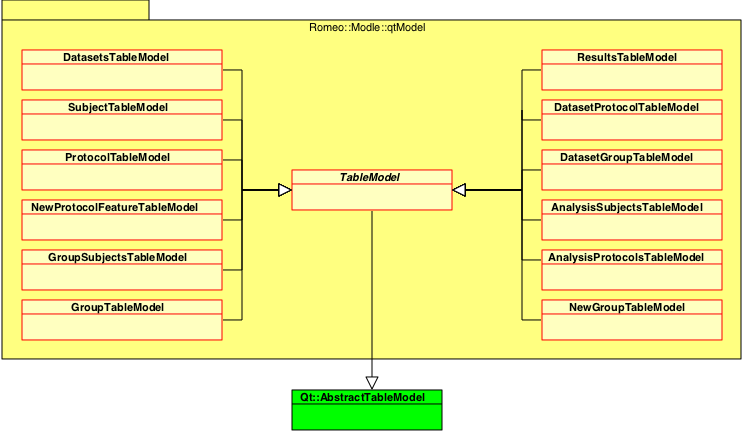
\includegraphics[width=\linewidth]{../Specifica_Tecnica/Content/Immagini/Romeo__Model__qtModel.png}
		\caption{Diagramma package \textsl{Romeo::Model::QtModel}}
		\label{comp_romeo_model_qtmodel}
	\end{figure}
	Package\g{} per il componente Model dell'architettura Model/View di Qt\g{}.
	
\subsubsection{TableModel(abstract)}
\label{TableModel}
\begin{figure}[!h]
	\centering
	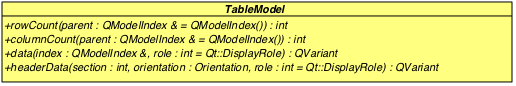
\includegraphics[width=0.6\linewidth]{./Content/Immagini/QtModel/TableModel.png}
	\caption{Diagramma classe \textsl{TableModel}}
	\label{comp_TableModel}
\end{figure}

\paragraph{Descrizione\\} 
Classe astratta che eredita da Qt::QAbstractTableModel.

\paragraph{Utilizzo\\}
La classe viene ereditata da tutte le classi che rappresentano i model delle tabelle visualizzate nelle view.

\paragraph{Classi ereditate:}
\begin{itemize}
	\item Qt::QAbstractTableModel.
\end{itemize}
	
\paragraph{\color{black}Metodi\\}
\begin{itemize}
	\item \color{blue}\verb!+ rowCount(parent : const QModelIndex &) : int!\\
	\color{black}
	\subparagraph{Descrizione:} metodo virtuale puro che ha come contratto il conteggio di numero di righe e lo ritorna.
	\\Il metodo viene invocato automaticamente da Qt\g{} nella generazione del Model.\\
	Il metodo deve essere ridefinito nelle classi che ereditano da questa.
	\subparagraph{Argomenti}
		\begin{itemize}
			\item \color{RoyalPurple}\verb!parent : const QModelIndex &!\\
			\color{Black}Rappresenta l'indice attuale del model.
		\end{itemize}
	\subparagraph{Note}
		\begin{itemize}
			\item Il metodo è costante puro e deve essere ridefinito dalle sottoclassi.
		\end{itemize}
	
	\item \color{blue}\verb!+ columnCount(parent : const QModelIndex &) : int!\\
	\color{black}
	\subparagraph{Descrizione:} metodo virtuale puro che ha come contratto il conteggio di numero di colonne e lo ritorna.\\
	Il metodo viene invocato automaticamente da Qt\g{} nella generazione del Model.\\
	Il metodo deve essere ridefinito nelle classi che ereditano da questa.\\
	\subparagraph{Argomenti}
		\begin{itemize}
			\item \color{RoyalPurple}\verb! parent : const QModelIndex &!\\
			\color{black}Rappresenta l'indice attuale del model.
		\end{itemize}
	\subparagraph{Note}
			\begin{itemize}
				\item Il metodo è costante puro e deve essere ridefinito dalle sottoclassi.
			\end{itemize}
		
	\item \color{blue}\verb! + data(index : const QModelIndex &, !\\
					\verb!role: int) : QVariant!\\
	\color{black}
	\subparagraph{Descrizione:} metodo virtuale puro che ha come contratto l'inserimento dei dati nella riga della tabella, ritorna il testo da inserire nelle singole celle\\
		Il metodo viene invocato automaticamente da Qt\g{} nella generazione del Model.\\
		Il metodo deve essere ridefinito nelle classi che ereditano da questa.\\
	\subparagraph{Argomenti}
		\begin{itemize}
			\item \color{RoyalPurple}\verb! parent : const QModelIndex &!\\
			\color{black}Rappresena l'indice attuale del model;
			
			\item \color{RoyalPurple}\verb! role : int!\\
			\color{black}Regola di visualizzazione Qt\g{}.
		\end{itemize}
	\subparagraph{Note}
			\begin{itemize}
				\item Il metodo è costante puro e deve essere ridefinito dalle sottoclassi.
			\end{itemize}
		
	\item \color{blue}\verb!+ headerData(section : int, orientation : Qt::Orientation,!\\
	  \verb!role : int) : QVariant!\\
	\color{black}
	\subparagraph{Descrizione:} metodo virtuale puro che ha come contratto l'inserimento delle intestazioni della tabella, ritorna il testo da inserire in ogni intestazione.\\
	Il metodo viene invocato automaticamente da Qt\g{} nella generazione del Model.\\
	Il metodo deve essere ridefinito nelle classi che ereditano da questa.\\
	\subparagraph{Argomenti}
		\begin{itemize}
			\item \color{RoyalPurple}\verb! section : int!\\
			\color{black}Rappresenta l'indice della colonna o riga in base all'orientamento;
			
			\item \color{RoyalPurple}\verb! orientation : Qt::Orientation!\\
			\color{black}Rappresenta l'orientamento della tabella;
			
			\item \color{RoyalPurple}\verb! role : int!\\
			\color{black}Regola di visualizzazione Qt\g{}.
		\end{itemize}
	\subparagraph{Note}
			\begin{itemize}
				\item Il metodo è costante puro e deve essere ridefinito dalle sottoclassi.
			\end{itemize}
\end{itemize}
\pagebreak

% % % % % % % % % % % % % % % % % % %

\subsubsection{AnalysisProtocolsTableModel(class)}
\label{AnalysisProtocolsTableModel}
\begin{figure}[!h]
	\centering
	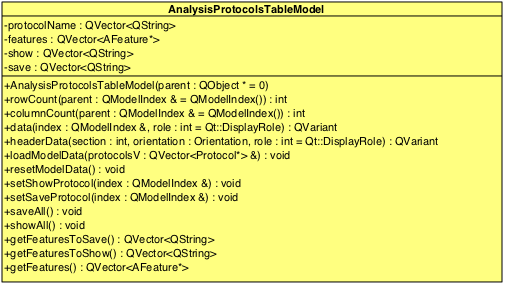
\includegraphics[width=0.6\linewidth]{./Content/Immagini/QtModel/AnalysisProtocolsTableModel.png}
	\caption{Diagramma classe \textsl{AnalysisProtocolsTableModel}}
	\label{comp_AnalysisProtocolsTableModel}
\end{figure}

\paragraph{Descrizione\\} 
Classe che rappresenta il model della tabella delle feature\g{} presente nella vista di avvio analisi.

\paragraph{Utilizzo\\}
La classe viene utilizzata come model dalla tabella delle feature\g{} della vista di avvio analisi.

\paragraph{Classi ereditate:}
\begin{itemize}
	\item Romeo::Model::QtModel::TableModel.
\end{itemize}

\paragraph{\textcolor{black}{Attributi\\}}
	\begin{itemize}
		\item \color{teal}\verb!- protocolName : QVector<QString>!
		\color{black}
		\subparagraph{Descrizione:} È il vettore dei nomi dei protocol\g{} presenti nel dataset\g{}.	
		\item \color{teal}\verb!- features : QVector<AFeature*>!
				\color{black}
				\subparagraph{Descrizione:} È il vettore delle feature\g{} che compone il model.				
		\item \color{teal}\verb!- show : QVector<QString>!
				\color{black}
				\subparagraph{Descrizione:} È il vettore di si e di no per le feature\g{} da mostrare durante l'analisi.				
		\item \color{teal}\verb!- save : QVector<QString>!
				\color{black}
				\subparagraph{Descrizione:} È il vettore di si e di no per le feature\g{} da esportare durante l'analisi.
	\end{itemize}
	
\paragraph{\color{black}Metodi\\}
\begin{itemize}
	\item \color{blue}\verb!+ AnalysisProtocolsTableModel(parent : QObject*)!\\
		\color{black}
		\subparagraph{Descrizione:} costruttore della classe.\\
		\subparagraph{Argomenti}
			\begin{itemize}
				\item \color{RoyalPurple}\verb!parent : QObject*!\\
				\color{Black}Parente dell'oggetto AnalysisProtocolsTableModel.
			\end{itemize}			
	\item \color{blue}\verb!+ rowCount(parent : const QModelIndex &) : int!\\
	\color{black}
	\subparagraph{Descrizione:} metodo virtuale che ha come contratto il conteggio di numero di righe e lo ritorna.
	\\Il metodo viene invocato automaticamente da Qt\g{} nella generazione del Model.
	\subparagraph{Argomenti}
		\begin{itemize}
			\item \color{RoyalPurple}\verb!parent : const QModelIndex &!\\
			\color{Black}Rappresenta l'indice attuale del model.
		\end{itemize}
	\subparagraph{Note}
		\begin{itemize}
			\item Il metodo è costante.
		\end{itemize}	
	\item \color{blue}\verb!+ columnCount(parent : const QModelIndex &) : int!\\
	\color{black}
	\subparagraph{Descrizione:} metodo virtuale che ha come contratto il conteggio di numero di colonne e lo ritorna. Il metodo viene invocato automaticamente da Qt\g{} nella generazione del Model. Il metodo deve essere ridefinito nelle classi che ereditano da questa.
	\subparagraph{Argomenti}
		\begin{itemize}
			\item \color{RoyalPurple}\verb! parent : const QModelIndex &!\\
			\color{black}Rappresenta l'indice attuale del model.
		\end{itemize}
	\subparagraph{Note}
			\begin{itemize}
				\item Il metodo è costante.
			\end{itemize}		
	\item \color{blue}\verb! + data(index : const QModelIndex &, !\\
					\verb!role: int) : QVariant!\\
	\color{black}
	\subparagraph{Descrizione:} metodo virtuale che ha come contratto l'inserimento dei dati nella riga della tabella, ritorna il testo da inserire nelle singole celle\\
		Il metodo viene invocato automaticamente da Qt\g{} nella generazione del Model.\\
		Il metodo deve essere ridefinito nelle classi che ereditano da questa.
	\subparagraph{Argomenti}
		\begin{itemize}
			\item \color{RoyalPurple}\verb! parent : const QModelIndex &!\\
			\color{black}Rappresena l'indice attuale del model;
			
			\item \color{RoyalPurple}\verb! role : int!\\
			\color{black}Regola di visualizzazione Qt\g{}.
		\end{itemize}
	\subparagraph{Note}
			\begin{itemize}
				\item Il metodo è costante.
			\end{itemize}		
	\item \color{blue}\verb!+ headerData(section : int, orientation : Qt::Orientation,!\\
	  \verb!role : int) : QVariant!\\
	\color{black}
	\subparagraph{Descrizione:} metodo virtuale che ha come contratto l'inserimento delle intestazioni della tabella, ritorna il testo da inserire in ogni intestazione.\\
	Il metodo viene invocato automaticamente da Qt\g{} nella generazione del Model.\\
	Il metodo deve essere ridefinito nelle classi che ereditano da questa.
	\subparagraph{Argomenti}
		\begin{itemize}
			\item \color{RoyalPurple}\verb! section : int!\\
			\color{black}Rappresenta l'indice della colonna o riga in base all'orientamento;
			
			\item \color{RoyalPurple}\verb! orientation : Qt::Orientation!\\
			\color{black}Rappresenta l'orientamento della tabella;
			
			\item \color{RoyalPurple}\verb! role : int!\\
			\color{black}Regola di visualizzazione Qt\g{}.
		\end{itemize}
	\subparagraph{Note}
			\begin{itemize}
				\item Il metodo è costante.
			\end{itemize}		
	\item \color{blue}\verb!+ loadModelData(protocolsV : const QVector<Protocol*>&) : void!\\
		\color{black}
		\subparagraph{Descrizione:} Carica i dati del model in base al nome del dataset\g{} passato come parametro al metodo.
		\subparagraph{Argomenti}
			\begin{itemize}				
				\item \color{RoyalPurple}\verb! protocolsV : const QVector<Protocol*>&!\\
				\color{black} Vettore dei protocol\g{} che andranno caricati nel model.
			\end{itemize}			
	\item \color{blue}\verb!+ resetModelData() : void!\\
		\color{black}
		\subparagraph{Descrizione:} Elimina i dati nel model portandolo allo stato vuoto.\\		
	\item \color{blue}\verb!+ setShowProtocol(index : const QModelIndex &) : void!\\
		\color{black}
		\subparagraph{Descrizione:} Imposta la feature\g{} puntata dall'indice come da visualizzare o no durante l'analisi.
		\subparagraph{Argomenti}
			\begin{itemize}				
				\item \color{RoyalPurple}\verb! index : const QModelIndex &!\\
				\color{black} Indice selezionato della tabella delle feature\g{}.
			\end{itemize}			
	\item \color{blue}\verb!+ setSaveProtocol(index : const QModelIndex &) : void!\\
		\color{black}
		\subparagraph{Descrizione:} Imposta la feature\g{} puntata dall'indice come da esportare o no durante l'analisi.
		\subparagraph{Argomenti}
			\begin{itemize}				
				\item \color{RoyalPurple}\verb! index : const QModelIndex &!\\
				\color{black} Indice selezionato della tabella delle feature\g{}.
			\end{itemize}			
	\item \color{blue}\verb!+ saveAll() : void!\\
		\color{black}
		\subparagraph{Descrizione:} Imposta tutte le feature\g{} come da esportare durante l'analisi.		
	\item \color{blue}\verb!+ showAll() : void!\\
		\color{black}
		\subparagraph{Descrizione:} Imposta tutte le feature\g{} come da visualizzare durante l'analisi.
	\item \color{blue}\verb!+ getFeaturesToSave() : QVector<QString>!\\
			\color{black}
			\subparagraph{Descrizione:} Il metodo ritorna il vettore delle feature\g{} da esportare durante l'analisi.
			\subparagraph{Note}
					\begin{itemize}
						\item Il metodo è costante.
					\end{itemize}					
	\item \color{blue}\verb!+ getFeaturesToShow() : QVector<QString>!\\
			\color{black}
			\subparagraph{Descrizione:} Il metodo ritorna il vettore delle feature\g{} da visualizzare durante l'analisi.
			\subparagraph{Note}
					\begin{itemize}
						\item Il metodo è costante.
					\end{itemize}						
	\item \color{blue}\verb!+ getFeatures() : QVector<AFeature*>!\\
			\color{black}
			\subparagraph{Descrizione:} Il metodo ritorna il vettore delle feature\g{} del model.
			\subparagraph{Note}
					\begin{itemize}
						\item Il metodo è costante.
					\end{itemize}
\end{itemize}
\pagebreak

% % % % % % % % % % % % % % % % % %

\subsubsection{AnalysisSubjectsTableModel(class)}
\label{AnalysisSubjectsTableModel}
\begin{figure}[!h]
	\centering
	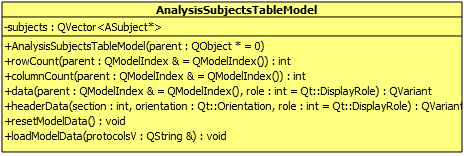
\includegraphics[width=0.6\linewidth]{./Content/Immagini/QtModel/AnalysisSubjectsTableModel.png}
	\caption{Diagramma classe \textsl{tAnalysisSubjectsTableModel}}
	\label{comp_AnalysisSubjectsTableModel}
\end{figure}

\paragraph{Descrizione\\} 
Classe che rappresenta il model della tabella dei subject\g{} presente nella vista di avvio analisi.

\paragraph{Utilizzo\\}
La classe viene utilizzata come model dalla tabella dei subject\g{} della vista di avvio analisi.

\paragraph{Classi ereditate:}
\begin{itemize}
	\item Romeo::Model::QtModel::TableModel.
\end{itemize}

\paragraph{\textcolor{black}{Attributi\\}}
	\begin{itemize}
		\item \color{teal}\verb!- subjects : QVector<ASubject*>!
		\color{black}
		\subparagraph{Descrizione:} È il vettore dei subject\g{} che compone il model.
	\end{itemize}
	
\paragraph{\color{black}Metodi\\}
\begin{itemize}
	\item \color{blue}\verb!+ AnalysisSubjectsTableModel(parent : QObject*)!\\
		\color{black}
		\subparagraph{Descrizione:} costruttore della classe.\\
		\subparagraph{Argomenti}
			\begin{itemize}
				\item \color{RoyalPurple}\verb!parent : QObject*!\\
				\color{Black}Parente dell'oggetto AnalysisSubjectsTableModel.
			\end{itemize}
				
	\item \color{blue}\verb!+ rowCount(parent : const QModelIndex &) : int!\\
	\color{black}
	\subparagraph{Descrizione:} metodo virtuale che ha come contratto il conteggio di numero di righe e lo ritorna.
	\\Il metodo viene invocato automaticamente da Qt\g{} nella generazione del Model.\\
	\subparagraph{Argomenti}
		\begin{itemize}
			\item \color{RoyalPurple}\verb!parent : const QModelIndex &!\\
			\color{Black}Rappresenta l'indice attuale del model.
		\end{itemize}
	\subparagraph{Note}
			\begin{itemize}
				\item Il metodo è costante.
			\end{itemize}
	
	\item \color{blue}\verb!+ columnCount(parent : const QModelIndex &) : int!\\
	\color{black}
	\subparagraph{Descrizione:} metodo virtuale che ha come contratto il conteggio di numero di colonne e lo ritorna.\\
	Il metodo viene invocato automaticamente da Qt\g{} nella generazione del Model.\\
	Il metodo deve essere ridefinito nelle classi che ereditano da questa.\\
	\subparagraph{Argomenti}
		\begin{itemize}
			\item \color{RoyalPurple}\verb! parent : const QModelIndex &!\\
			\color{black}Rappresenta l'indice attuale del model.
		\end{itemize}
	\subparagraph{Note}
			\begin{itemize}
				\item Il metodo è costante.
			\end{itemize}
		
	\item \color{blue}\verb! + data(index : const QModelIndex &, !\\
					\verb!role: int) : QVariant!\\
	\color{black}
	\subparagraph{Descrizione:} metodo virtuale che ha come contratto l'inserimento dei dati nella riga della tabella, ritorna il testo da inserire nelle singole celle\\
		Il metodo viene invocato automaticamente da Qt\g{} nella generazione del Model.\\
		Il metodo deve essere ridefinito nelle classi che ereditano da questa.\\
	\subparagraph{Argomenti}
		\begin{itemize}
			\item \color{RoyalPurple}\verb! parent : const QModelIndex &!\\
			\color{black}Rappresena l'indice attuale del model;
			
			\item \color{RoyalPurple}\verb! role : int!\\
			\color{black}Regola di visualizzazione Qt\g{}.
		\end{itemize}
	\subparagraph{Note}
			\begin{itemize}
				\item Il metodo è costante.
			\end{itemize}
		
	\item \color{blue}\verb!+ headerData(section : int, orientation : Qt::Orientation,!\\
	  \verb!role : int) : QVariant!\\
	\color{black}
	\subparagraph{Descrizione:} metodo virtuale che ha come contratto l'inserimento delle intestazioni della tabella, ritorna il testo da inserire in ogni intestazione.\\
	Il metodo viene invocato automaticamente da Qt\g{} nella generazione del Model.\\
	Il metodo deve essere ridefinito nelle classi che ereditano da questa.\\
	\subparagraph{Argomenti}
		\begin{itemize}
			\item \color{RoyalPurple}\verb! section : int!\\
			\color{black}Rappresenta l'indice della colonna o riga in base all'orientamento;
			
			\item \color{RoyalPurple}\verb! orientation : Qt::Orientation!\\
			\color{black}Rappresenta l'orientamento della tabella;
			
			\item \color{RoyalPurple}\verb! role : int!\\
			\color{black}Regola di visualizzazione Qt\g{}.
		\end{itemize}
	\subparagraph{Note}
			\begin{itemize}
				\item Il metodo è costante.
			\end{itemize}
		
	\item \color{blue}\verb!+ loadModelData(dataset : const QString&) : void!\\
		\color{black}
		\subparagraph{Descrizione:} Carica i dati del model in base al nome del dataset\g{} passato come parametro al metodo.\\
		\subparagraph{Argomenti}
			\begin{itemize}				
				\item \color{RoyalPurple}\verb! dataset : const QString&!\\
				\color{black} Nome del dataset\g{}.
			\end{itemize}
			
	\item \color{blue}\verb!+ resetModelData() : void!\\
			\color{black}
			\subparagraph{Descrizione:} Elimina i dati nel model portandolo allo stato vuoto.\\
\end{itemize}
\pagebreak

% % % % % % % % % % % % % % % % % %

\subsubsection{DatasetGroupTableModel(class)}
\label{DatasetGroupTableModel}
\begin{figure}[!h]
	\centering
	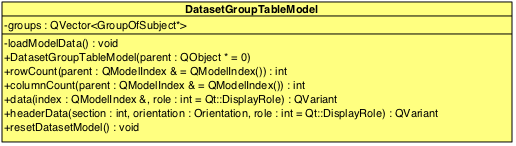
\includegraphics[width=0.6\linewidth]{./Content/Immagini/QtModel/DatasetGroupTableModel.png}
	\caption{Diagramma classe \textsl{DatasetGroupTableModel}}
	\label{comp_DatasetGroupTableModel}
\end{figure}

\paragraph{Descrizione\\} 
Classe che rappresenta il model della tabella dei gruppi di subject\g{} presente nella vista di creazione del dataset\g{}.

\paragraph{Utilizzo\\}
La classe viene utilizzata come model dalla tabella dei gruppi di subject\g{} della vista di creazione del dataset\g{}.

\paragraph{Classi ereditate:}
\begin{itemize}
	\item Romeo::Model::QtModel::TableModel.
\end{itemize}

\paragraph{\textcolor{black}{Attributi\\}}
	\begin{itemize}
		\item \color{teal}\verb!- groups : QVector<GroupOfSubject*>!
		\color{black}
		\subparagraph{Descrizione:} È il vettore dei gruppi di subject\g{} che compone il model.
	\end{itemize}
	
\paragraph{\color{black}Metodi\\}
\begin{itemize}
	\item \color{blue}\verb!+ DatasetGroupTableModel(parent : QObject*)!\\
		\color{black}
		\subparagraph{Descrizione:} costruttore della classe.\\
		\subparagraph{Argomenti}
			\begin{itemize}
				\item \color{RoyalPurple}\verb!parent : QObject*!\\
				\color{Black}Parente dell'oggetto DatasetGroupTableModel.
			\end{itemize}
			
	\item \color{blue}\verb!+ rowCount(parent : const QModelIndex &) : int!\\
	\color{black}
	\subparagraph{Descrizione:} metodo virtuale che ha come contratto il conteggio di numero di righe e lo ritorna.
	\\Il metodo viene invocato automaticamente da Qt\g{} nella generazione del Model.\\
	\subparagraph{Argomenti}
		\begin{itemize}
			\item \color{RoyalPurple}\verb!parent : const QModelIndex &!\\
			\color{Black}Rappresenta l'indice attuale del model.
		\end{itemize}
	\subparagraph{Note}
			\begin{itemize}
				\item Il metodo è costante.
			\end{itemize}
	
	\item \color{blue}\verb!+ columnCount(parent : const QModelIndex &) : int!\\
	\color{black}
	\subparagraph{Descrizione:} metodo virtuale che ha come contratto il conteggio di numero di colonne e lo ritorna.\\
	Il metodo viene invocato automaticamente da Qt\g{} nella generazione del Model.\\
	Il metodo deve essere ridefinito nelle classi che ereditano da questa.\\
	\subparagraph{Argomenti}
		\begin{itemize}
			\item \color{RoyalPurple}\verb! parent : const QModelIndex &!\\
			\color{black}Rappresenta l'indice attuale del model.
		\end{itemize}
	\subparagraph{Note}
			\begin{itemize}
				\item Il metodo è costante.
			\end{itemize}
		
	\item \color{blue}\verb! + data(index : const QModelIndex &, !\\
					\verb!role: int) : QVariant!\\
	\color{black}
	\subparagraph{Descrizione:} metodo virtuale che ha come contratto l'inserimento dei dati nella riga della tabella, ritorna il testo da inserire nelle singole celle\\
		Il metodo viene invocato automaticamente da Qt\g{} nella generazione del Model.\\
		Il metodo deve essere ridefinito nelle classi che ereditano da questa.\\
	\subparagraph{Argomenti}
		\begin{itemize}
			\item \color{RoyalPurple}\verb! parent : const QModelIndex &!\\
			\color{black}Rappresena l'indice attuale del model;
			
			\item \color{RoyalPurple}\verb! role : int!\\
			\color{black}Regola di visualizzazione Qt\g{}.
		\end{itemize}
	\subparagraph{Note}
			\begin{itemize}
				\item Il metodo è costante.
			\end{itemize}
		
	\item \color{blue}\verb!+ headerData(section : int, orientation : Qt::Orientation,!\\
	  \verb!role : int) : QVariant!\\
	\color{black}
	\subparagraph{Descrizione:} metodo virtuale che ha come contratto l'inserimento delle intestazioni della tabella, ritorna il testo da inserire in ogni intestazione.\\
	Il metodo viene invocato automaticamente da Qt\g{} nella generazione del Model.\\
	Il metodo deve essere ridefinito nelle classi che ereditano da questa.\\
	\subparagraph{Argomenti}
		\begin{itemize}
			\item \color{RoyalPurple}\verb! section : int!\\
			\color{black}Rappresenta l'indice della colonna o riga in base all'orientamento;
			
			\item \color{RoyalPurple}\verb! orientation : Qt::Orientation!\\
			\color{black}Rappresenta l'orientamento della tabella;
			
			\item \color{RoyalPurple}\verb! role : int!\\
			\color{black}Regola di visualizzazione Qt\g{}.
		\end{itemize}
	\subparagraph{Note}
			\begin{itemize}
				\item Il metodo è costante.
			\end{itemize}
		
	\item \color{blue}\verb!+ resetDatasetModel() : void!\\
		\color{black}
		\subparagraph{Descrizione:} Elimina i dati nel model portandolo allo stato vuoto.\\
			
	\item \color{blue}\verb!- loadModelData() : void!\\
		\color{black}
		\subparagraph{Descrizione:} Carica i dati del model .\\
\end{itemize}
\pagebreak

% % % % % % % % % % % % % % % % % %

\subsubsection{DatasetProtocolTableModel(class)}
\label{DatasetProtocolTableModel}
\begin{figure}[!h]
	\centering
	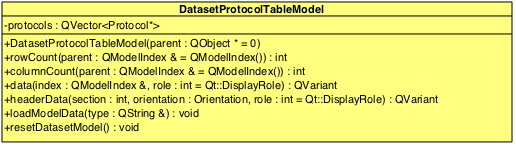
\includegraphics[width=0.6\linewidth]{./Content/Immagini/QtModel/DatasetProtocolTableModel.png}
	\caption{Diagramma classe \textsl{DatasetProtocolTableModel}}
	\label{comp_DatasetProtocolTableModel}
\end{figure}

\paragraph{Descrizione\\} 
Classe che rappresenta il model della tabella dei protocol\g{} presente nella vista di creazione dei dataset\g{}.

\paragraph{Utilizzo\\}
La classe viene utilizzata come model dalla tabella dei protocol\g{} della vista di creazione dei dataset\g{}.

\paragraph{Classi ereditate:}
\begin{itemize}
	\item Romeo::Model::QtModel::TableModel.
\end{itemize}

\paragraph{\textcolor{black}{Attributi\\}}
	\begin{itemize}
		\item \color{teal}\verb!- protocols : QVector<Protocol*>!
		\color{black}
		\subparagraph{Descrizione:} È il vettore dei protocol\g{} che compone il model.
	\end{itemize}
	
\paragraph{\color{black}Metodi\\}
\begin{itemize}
	\item \color{blue}\verb!+ DatasetProtocolTableModel(parent : QObject*)!\\
		\color{black}
		\subparagraph{Descrizione:} costruttore della classe.\\
		\subparagraph{Argomenti}
			\begin{itemize}
				\item \color{RoyalPurple}\verb!parent : QObject*!\\
				\color{Black}Parente dell'oggetto DatasetProtocolTableModel.
			\end{itemize}
			
	\item \color{blue}\verb!+ rowCount(parent : const QModelIndex &) : int!\\
	\color{black}
	\subparagraph{Descrizione:} metodo virtuale che ha come contratto il conteggio di numero di righe e lo ritorna.
	\\Il metodo viene invocato automaticamente da Qt\g{} nella generazione del Model.\\
	\subparagraph{Argomenti}
		\begin{itemize}
			\item \color{RoyalPurple}\verb!parent : const QModelIndex &!\\
			\color{Black}Rappresenta l'indice attuale del model.
		\end{itemize}
	\subparagraph{Note}
			\begin{itemize}
				\item Il metodo è costante.
			\end{itemize}
	
	\item \color{blue}\verb!+ columnCount(parent : const QModelIndex &) : int!\\
	\color{black}
	\subparagraph{Descrizione:} metodo virtuale che ha come contratto il conteggio di numero di colonne e lo ritorna.\\
	Il metodo viene invocato automaticamente da Qt\g{} nella generazione del Model.\\
	Il metodo deve essere ridefinito nelle classi che ereditano da questa.\\
	\subparagraph{Argomenti}
		\begin{itemize}
			\item \color{RoyalPurple}\verb! parent : const QModelIndex &!\\
			\color{black}Rappresenta l'indice attuale del model.
		\end{itemize}
	\subparagraph{Note}
			\begin{itemize}
				\item Il metodo è costante.
			\end{itemize}
		
	\item \color{blue}\verb! + data(index : const QModelIndex &, !\\
					\verb!role: int) : QVariant!\\
	\color{black}
	\subparagraph{Descrizione:} metodo virtuale che ha come contratto l'inserimento dei dati nella riga della tabella, ritorna il testo da inserire nelle singole celle\\
		Il metodo viene invocato automaticamente da Qt\g{} nella generazione del Model.\\
		Il metodo deve essere ridefinito nelle classi che ereditano da questa.\\
	\subparagraph{Argomenti}
		\begin{itemize}
			\item \color{RoyalPurple}\verb! parent : const QModelIndex &!\\
			\color{black}Rappresena l'indice attuale del model;
			
			\item \color{RoyalPurple}\verb! role : int!\\
			\color{black}Regola di visualizzazione Qt\g{}.
		\end{itemize}
	\subparagraph{Note}
			\begin{itemize}
				\item Il metodo è costante.
			\end{itemize}
		
	\item \color{blue}\verb!+ headerData(section : int, orientation : Qt::Orientation,!\\
	  \verb!role : int) : QVariant!\\
	\color{black}
	\subparagraph{Descrizione:} metodo virtuale che ha come contratto l'inserimento delle intestazioni della tabella, ritorna il testo da inserire in ogni intestazione.\\
	Il metodo viene invocato automaticamente da Qt\g{} nella generazione del Model.\\
	Il metodo deve essere ridefinito nelle classi che ereditano da questa.\\
	\subparagraph{Argomenti}
		\begin{itemize}
			\item \color{RoyalPurple}\verb! section : int!\\
			\color{black}Rappresenta l'indice della colonna o riga in base all'orientamento;
			
			\item \color{RoyalPurple}\verb! orientation : Qt::Orientation!\\
			\color{black}Rappresenta l'orientamento della tabella;
			
			\item \color{RoyalPurple}\verb! role : int!\\
			\color{black}Regola di visualizzazione Qt\g{}.
		\end{itemize}
	\subparagraph{Note}
			\begin{itemize}
				\item Il metodo è costante.
			\end{itemize}
		
	\item \color{blue}\verb!+ loadModelData(type : const QString&) : void!\\
		\color{black}
		\subparagraph{Descrizione:} Carica i dati del model in base al tipo passato come parametro al metodo.\\
		\subparagraph{Argomenti}
			\begin{itemize}				
				\item \color{RoyalPurple}\verb! type : const QString&!\\
				\color{black} Tipo del protocol\g{}.
			\end{itemize}
			
	\item \color{blue}\verb!+ resetDatasetModel() : void!\\
		\color{black}
		\subparagraph{Descrizione:} Elimina i dati nel model portandolo allo stato vuoto.\\
\end{itemize}
\pagebreak

% % % % % % % % % % % % % % % % % %

\subsubsection{DatasetsTableModel(class)}
\label{DatasetsTableModel}
\begin{figure}[!h]
	\centering
	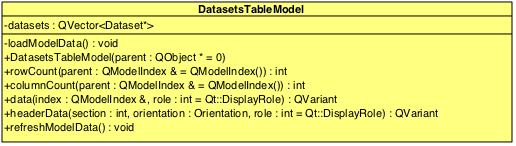
\includegraphics[width=0.6\linewidth]{./Content/Immagini/QtModel/DatasetsTableModel.png}
	\caption{Diagramma classe \textsl{DatasetsTableModel}}
	\label{comp_DatasetsTableModel}
\end{figure}

\paragraph{Descrizione\\} 
Classe che rappresenta il model della tabella dei dataset\g{} presente nella vista di visualizzazione dei dataset\g{}.

\paragraph{Utilizzo\\}
La classe viene utilizzata come model dalla tabella dei dataset\g{ della vista di visualizzazione dei dataset\g{}.

\paragraph{Classi ereditate:}
\begin{itemize}
	\item Romeo::Model::QtModel::TableModel.
\end{itemize}

\paragraph{\textcolor{black}{Attributi\\}}
	\begin{itemize}
		\item \color{teal}\verb!- datasets : QVector<Dataset*>!
		\color{black}
		\subparagraph{Descrizione:} È il vettore dei dataset\g{} che compone il model.
	\end{itemize}
	
\paragraph{\color{black}Metodi\\}
\begin{itemize}
	\item \color{blue}\verb!+ DatasetsTableModel(parent : QObject*)!\\
		\color{black}
		\subparagraph{Descrizione:} costruttore della classe.\\
		\subparagraph{Argomenti}
			\begin{itemize}
				\item \color{RoyalPurple}\verb!parent : QObject*!\\
				\color{Black}Parente dell'oggetto DatasetsTableModel.
			\end{itemize}
			
	\item \color{blue}\verb!+ rowCount(parent : const QModelIndex &) : int!\\
	\color{black}
	\subparagraph{Descrizione:} metodo virtuale che ha come contratto il conteggio di numero di righe e lo ritorna.
	\\Il metodo viene invocato automaticamente da Qt\g{} nella generazione del Model.\\
	\subparagraph{Argomenti}
		\begin{itemize}
			\item \color{RoyalPurple}\verb!parent : const QModelIndex &!\\
			\color{Black}Rappresenta l'indice attuale del model.
		\end{itemize}
	\subparagraph{Note}
			\begin{itemize}
				\item Il metodo è costante.
			\end{itemize}
	
	\item \color{blue}\verb!+ columnCount(parent : const QModelIndex &) : int!\\
	\color{black}
	\subparagraph{Descrizione:} metodo virtuale che ha come contratto il conteggio di numero di colonne e lo ritorna.\\
	Il metodo viene invocato automaticamente da Qt\g{} nella generazione del Model.\\
	Il metodo deve essere ridefinito nelle classi che ereditano da questa.\\
	\subparagraph{Argomenti}
		\begin{itemize}
			\item \color{RoyalPurple}\verb! parent : const QModelIndex &!\\
			\color{black}Rappresenta l'indice attuale del model.
		\end{itemize}
	\subparagraph{Note}
			\begin{itemize}
				\item Il metodo è costante.
			\end{itemize}
		
	\item \color{blue}\verb! + data(index : const QModelIndex &, !\\
					\verb!role: int) : QVariant!\\
	\color{black}
	\subparagraph{Descrizione:} metodo virtuale che ha come contratto l'inserimento dei dati nella riga della tabella, ritorna il testo da inserire nelle singole celle\\
		Il metodo viene invocato automaticamente da Qt\g{} nella generazione del Model.\\
		Il metodo deve essere ridefinito nelle classi che ereditano da questa.\\
	\subparagraph{Argomenti}
		\begin{itemize}
			\item \color{RoyalPurple}\verb! parent : const QModelIndex &!\\
			\color{black}Rappresena l'indice attuale del model;
			
			\item \color{RoyalPurple}\verb! role : int!\\
			\color{black}Regola di visualizzazione Qt\g{}.
		\end{itemize}
	\subparagraph{Note}
			\begin{itemize}
				\item Il metodo è costante.
			\end{itemize}
		
	\item \color{blue}\verb!+ headerData(section : int, orientation : Qt::Orientation,!\\
	  \verb!role : int) : QVariant!\\
	\color{black}
	\subparagraph{Descrizione:} metodo virtuale che ha come contratto l'inserimento delle intestazioni della tabella, ritorna il testo da inserire in ogni intestazione.\\
	Il metodo viene invocato automaticamente da Qt\g{} nella generazione del Model.\\
	Il metodo deve essere ridefinito nelle classi che ereditano da questa.\\
	\subparagraph{Argomenti}
		\begin{itemize}
			\item \color{RoyalPurple}\verb! section : int!\\
			\color{black}Rappresenta l'indice della colonna o riga in base all'orientamento;
			
			\item \color{RoyalPurple}\verb! orientation : Qt::Orientation!\\
			\color{black}Rappresenta l'orientamento della tabella;
			
			\item \color{RoyalPurple}\verb! role : int!\\
			\color{black}Regola di visualizzazione Qt\g{}.
		\end{itemize}
	\subparagraph{Note}
			\begin{itemize}
				\item Il metodo è costante.
			\end{itemize}
		
	\item \color{blue}\verb!+ refreshModelData() : void!\\
		\color{black}
		\subparagraph{Descrizione:} Ricarica i dati del model.\\
			
	\item \color{blue}\verb!- loadModelData() : void!\\
		\color{black}
		\subparagraph{Descrizione:} Carica i dati del model .\\
\end{itemize}
\pagebreak

% % % % % % % % % % % % % % % % % %

\subsubsection{GroupSubjectsTableModel(class)}
\label{GroupSubjectsTableModel}
\begin{figure}[!h]
	\centering
	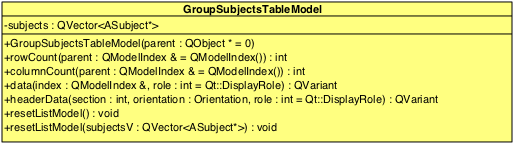
\includegraphics[width=0.6\linewidth]{./Content/Immagini/QtModel/GroupSubjectsTableModel.png}
	\caption{Diagramma classe \textsl{GroupSubjectsTableModel}}
	\label{comp_GroupSubjectsTableModel}
\end{figure}

\paragraph{Descrizione\\} 
Classe che rappresenta il model della tabella dei subject\g{} presente nella vista di visualizzazione dei gruppi di subject\g{}.

\paragraph{Utilizzo\\}
La classe viene utilizzata come model dalla tabella dei subject\g{} della vista di visualizzazione dei gruppi di subject\g{}.

\paragraph{Classi ereditate:}
\begin{itemize}
	\item Romeo::Model::QtModel::TableModel.
\end{itemize}

\paragraph{\textcolor{black}{Attributi\\}}
	\begin{itemize}
		\item \color{teal}\verb!- subjects : QVector<ASubject*>!
		\color{black}
		\subparagraph{Descrizione:} È il vettore dei subject\g{} che compone il model.
	\end{itemize}
	
\paragraph{\color{black}Metodi\\}
\begin{itemize}
	\item \color{blue}\verb!+ GroupSubjectsTableModel(parent : QObject*)!\\
		\color{black}
		\subparagraph{Descrizione:} costruttore della classe.\\
		\subparagraph{Argomenti}
			\begin{itemize}
				\item \color{RoyalPurple}\verb!parent : QObject*!\\
				\color{Black}Parente dell'oggetto GroupSubjectsTableModel.
			\end{itemize}
			
	\item \color{blue}\verb!+ rowCount(parent : const QModelIndex &) : int!\\
	\color{black}
	\subparagraph{Descrizione:} metodo virtuale che ha come contratto il conteggio di numero di righe e lo ritorna.
	\\Il metodo viene invocato automaticamente da Qt\g{} nella generazione del Model.\\
	\subparagraph{Argomenti}
		\begin{itemize}
			\item \color{RoyalPurple}\verb!parent : const QModelIndex &!\\
			\color{Black}Rappresenta l'indice attuale del model.
		\end{itemize}
	\subparagraph{Note}
			\begin{itemize}
				\item Il metodo è costante.
			\end{itemize}
	
	\item \color{blue}\verb!+ columnCount(parent : const QModelIndex &) : int!\\
	\color{black}
	\subparagraph{Descrizione:} metodo virtuale che ha come contratto il conteggio di numero di colonne e lo ritorna.\\
	Il metodo viene invocato automaticamente da Qt\g{} nella generazione del Model.\\
	Il metodo deve essere ridefinito nelle classi che ereditano da questa.\\
	\subparagraph{Argomenti}
		\begin{itemize}
			\item \color{RoyalPurple}\verb! parent : const QModelIndex &!\\
			\color{black}Rappresenta l'indice attuale del model.
		\end{itemize}
	\subparagraph{Note}
			\begin{itemize}
				\item Il metodo è costante.
			\end{itemize}
		
	\item \color{blue}\verb! + data(index : const QModelIndex &, !\\
					\verb!role: int) : QVariant!\\
	\color{black}
	\subparagraph{Descrizione:} metodo virtuale che ha come contratto l'inserimento dei dati nella riga della tabella, ritorna il testo da inserire nelle singole celle\\
		Il metodo viene invocato automaticamente da Qt\g{} nella generazione del Model.\\
		Il metodo deve essere ridefinito nelle classi che ereditano da questa.\\
	\subparagraph{Argomenti}
		\begin{itemize}
			\item \color{RoyalPurple}\verb! parent : const QModelIndex &!\\
			\color{black}Rappresena l'indice attuale del model;
			
			\item \color{RoyalPurple}\verb! role : int!\\
			\color{black}Regola di visualizzazione Qt\g{}.
		\end{itemize}
	\subparagraph{Note}
			\begin{itemize}
				\item Il metodo è costante.
			\end{itemize}
		
	\item \color{blue}\verb!+ headerData(section : int, orientation : Qt::Orientation,!\\
	  \verb!role : int) : QVariant!\\
	\color{black}
	\subparagraph{Descrizione:} metodo virtuale che ha come contratto l'inserimento delle intestazioni della tabella, ritorna il testo da inserire in ogni intestazione.\\
	Il metodo viene invocato automaticamente da Qt\g{} nella generazione del Model.\\
	Il metodo deve essere ridefinito nelle classi che ereditano da questa.\\
	\subparagraph{Argomenti}
		\begin{itemize}
			\item \color{RoyalPurple}\verb! section : int!\\
			\color{black}Rappresenta l'indice della colonna o riga in base all'orientamento;
			
			\item \color{RoyalPurple}\verb! orientation : Qt::Orientation!\\
			\color{black}Rappresenta l'orientamento della tabella;
			
			\item \color{RoyalPurple}\verb! role : int!\\
			\color{black}Regola di visualizzazione Qt\g{}.
		\end{itemize}
	\subparagraph{Note}
			\begin{itemize}
				\item Il metodo è costante.
			\end{itemize}
		
	\item \color{blue}\verb!+ resetListModel(subjectsV : QVector<ASubject*>) : void!\\
		\color{black}
		\subparagraph{Descrizione:} Carica i dati del model con i dati passati come parametro al metodo.\\
		\subparagraph{Argomenti}
			\begin{itemize}				
				\item \color{RoyalPurple}\verb! subjectsV : QVector<ASubject*>!\\
				\color{black} Vettore di subject\g{}.
			\end{itemize}
			
	\item \color{blue}\verb!+ resetListModel() : void!\\
		\color{black}
		\subparagraph{Descrizione:} Ricarica i dati nel model.\\
\end{itemize}
\pagebreak

% % % % % % % % % % % % % % % % % %

\subsubsection{GroupTableModel(class)}
\label{GroupTableModel}
\begin{figure}[!h]
	\centering
	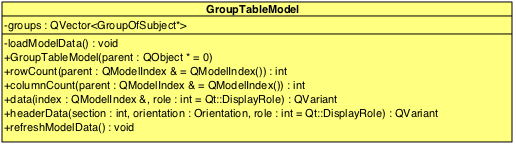
\includegraphics[width=0.6\linewidth]{./Content/Immagini/QtModel/GroupTableModel.png}
	\caption{Diagramma classe \textsl{GroupTableModel}}
	\label{comp_GroupTableModel}
\end{figure}

\paragraph{Descrizione\\} 
Classe che rappresenta il model della tabella dei gruppi di subject\g{} presente nella vista di visualizzazione dei gruppi di subject\g{}.

\paragraph{Utilizzo\\}
La classe viene utilizzata come model dalla tabella dei gruppi di subject\g{} della vista di visualizzazione dei gruppi di subject\g{}.

\paragraph{Classi ereditate:}
\begin{itemize}
	\item Romeo::Model::QtModel::TableModel.
\end{itemize}

\paragraph{\textcolor{black}{Attributi\\}}
	\begin{itemize}
		\item \color{teal}\verb!- groups : QVector<GroupOfSubject*>!
		\color{black}
		\subparagraph{Descrizione:} È il vettore dei gruppi di subject\g{} che compone il model.
	\end{itemize}
	
\paragraph{\color{black}Metodi\\}
\begin{itemize}
	\item \color{blue}\verb!+ GroupTableModel(parent : QObject*)!\\
		\color{black}
		\subparagraph{Descrizione:} costruttore della classe.\\
		\subparagraph{Argomenti}
			\begin{itemize}
				\item \color{RoyalPurple}\verb!parent : QObject*!\\
				\color{Black}Parente dell'oggetto GroupTableModel.
			\end{itemize}
			
	\item \color{blue}\verb!+ rowCount(parent : const QModelIndex &) : int!\\
	\color{black}
	\subparagraph{Descrizione:} metodo virtuale che ha come contratto il conteggio di numero di righe e lo ritorna.
	\\Il metodo viene invocato automaticamente da Qt\g{} nella generazione del Model.\\
	\subparagraph{Argomenti}
		\begin{itemize}
			\item \color{RoyalPurple}\verb!parent : const QModelIndex &!\\
			\color{Black}Rappresenta l'indice attuale del model.
		\end{itemize}
	\subparagraph{Note}
			\begin{itemize}
				\item Il metodo è costante.
			\end{itemize}
	
	\item \color{blue}\verb!+ columnCount(parent : const QModelIndex &) : int!\\
	\color{black}
	\subparagraph{Descrizione:} metodo virtuale che ha come contratto il conteggio di numero di colonne e lo ritorna.\\
	Il metodo viene invocato automaticamente da Qt\g{} nella generazione del Model.\\
	Il metodo deve essere ridefinito nelle classi che ereditano da questa.\\
	\subparagraph{Argomenti}
		\begin{itemize}
			\item \color{RoyalPurple}\verb! parent : const QModelIndex &!\\
			\color{black}Rappresenta l'indice attuale del model.
		\end{itemize}
	\subparagraph{Note}
			\begin{itemize}
				\item Il metodo è costante.
			\end{itemize}
		
	\item \color{blue}\verb! + data(index : const QModelIndex &, !\\
					\verb!role: int) : QVariant!\\
	\color{black}
	\subparagraph{Descrizione:} metodo virtuale che ha come contratto l'inserimento dei dati nella riga della tabella, ritorna il testo da inserire nelle singole celle\\
		Il metodo viene invocato automaticamente da Qt\g{} nella generazione del Model.\\
		Il metodo deve essere ridefinito nelle classi che ereditano da questa.\\
	\subparagraph{Argomenti}
		\begin{itemize}
			\item \color{RoyalPurple}\verb! parent : const QModelIndex &!\\
			\color{black}Rappresena l'indice attuale del model;
			
			\item \color{RoyalPurple}\verb! role : int!\\
			\color{black}Regola di visualizzazione Qt\g{}.
		\end{itemize}
	\subparagraph{Note}
			\begin{itemize}
				\item Il metodo è costante.
			\end{itemize}
		
	\item \color{blue}\verb!+ headerData(section : int, orientation : Qt::Orientation,!\\
	  \verb!role : int) : QVariant!\\
	\color{black}
	\subparagraph{Descrizione:} metodo virtuale che ha come contratto l'inserimento delle intestazioni della tabella, ritorna il testo da inserire in ogni intestazione.\\
	Il metodo viene invocato automaticamente da Qt\g{} nella generazione del Model.\\
	Il metodo deve essere ridefinito nelle classi che ereditano da questa.\\
	\subparagraph{Argomenti}
		\begin{itemize}
			\item \color{RoyalPurple}\verb! section : int!\\
			\color{black}Rappresenta l'indice della colonna o riga in base all'orientamento;
			
			\item \color{RoyalPurple}\verb! orientation : Qt::Orientation!\\
			\color{black}Rappresenta l'orientamento della tabella;
			
			\item \color{RoyalPurple}\verb! role : int!\\
			\color{black}Regola di visualizzazione Qt\g{}.
		\end{itemize}
	\subparagraph{Note}
			\begin{itemize}
				\item Il metodo è costante.
			\end{itemize}
		
	\item \color{blue}\verb!+ refreshModelData() : void!\\
		\color{black}
		\subparagraph{Descrizione:} Ricarica i dati del model.\\
			
	\item \color{blue}\verb!- loadModelData() : void!\\
		\color{black}
		\subparagraph{Descrizione:} Carica i dati del model .\\
\end{itemize}
\pagebreak

% % % % % % % % % % % % % % % % % %

\subsubsection{NewGroupTableModel(class)}
\label{NewGroupTableModel}
\begin{figure}[!h]
	\centering
	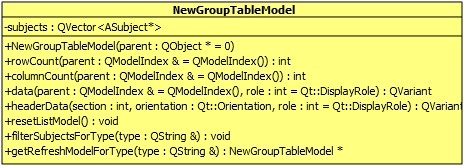
\includegraphics[width=0.6\linewidth]{./Content/Immagini/QtModel/NewGroupTableModel.png}
	\caption{Diagramma classe \textsl{NewGroupTableModel}}
	\label{comp_NewGroupTableModel}
\end{figure}

\paragraph{Descrizione\\} 
Classe che rappresenta il model della tabella dei subject\g{} presente nella vista di creazione dei gruppi di subject\g{}.

\paragraph{Utilizzo\\}
La classe viene utilizzata come model dalla tabella dei subject\g{} della vista di creazione dei gruppi di subject\g{}.

\paragraph{Classi ereditate:}
\begin{itemize}
	\item Romeo::Model::QtModel::TableModel.
\end{itemize}

\paragraph{\textcolor{black}{Attributi\\}}
	\begin{itemize}
		\item \color{teal}\verb!- subjects : QVector<ASubject*>!
		\color{black}
		\subparagraph{Descrizione:} È il vettore dei subject\g{} che compone il model.
	\end{itemize}
	
\paragraph{\color{black}Metodi\\}
\begin{itemize}
	\item \color{blue}\verb!+ NewGroupTableModel(parent : QObject*)!\\
		\color{black}
		\subparagraph{Descrizione:} costruttore della classe.\\
		\subparagraph{Argomenti}
			\begin{itemize}
				\item \color{RoyalPurple}\verb!parent : QObject*!\\
				\color{Black}Parente dell'oggetto NewGroupTableModel.
			\end{itemize}
			
	\item \color{blue}\verb!+ rowCount(parent : const QModelIndex &) : int!\\
	\color{black}
	\subparagraph{Descrizione:} metodo virtuale che ha come contratto il conteggio di numero di righe e lo ritorna.
	\\Il metodo viene invocato automaticamente da Qt\g{} nella generazione del Model.\\
	\subparagraph{Argomenti}
		\begin{itemize}
			\item \color{RoyalPurple}\verb!parent : const QModelIndex &!\\
			\color{Black}Rappresenta l'indice attuale del model.
		\end{itemize}
	\subparagraph{Note}
			\begin{itemize}
				\item Il metodo è costante.
			\end{itemize}
	
	\item \color{blue}\verb!+ columnCount(parent : const QModelIndex &) : int!\\
	\color{black}
	\subparagraph{Descrizione:} metodo virtuale che ha come contratto il conteggio di numero di colonne e lo ritorna.\\
	Il metodo viene invocato automaticamente da Qt\g{} nella generazione del Model.\\
	Il metodo deve essere ridefinito nelle classi che ereditano da questa.\\
	\subparagraph{Argomenti}
		\begin{itemize}
			\item \color{RoyalPurple}\verb! parent : const QModelIndex &!\\
			\color{black}Rappresenta l'indice attuale del model.
		\end{itemize}
	\subparagraph{Note}
			\begin{itemize}
				\item Il metodo è costante.
			\end{itemize}
		
	\item \color{blue}\verb! + data(index : const QModelIndex &, !\\
					\verb!role: int) : QVariant!\\
	\color{black}
	\subparagraph{Descrizione:} metodo virtuale che ha come contratto l'inserimento dei dati nella riga della tabella, ritorna il testo da inserire nelle singole celle\\
		Il metodo viene invocato automaticamente da Qt\g{} nella generazione del Model.\\
		Il metodo deve essere ridefinito nelle classi che ereditano da questa.\\
	\subparagraph{Argomenti}
		\begin{itemize}
			\item \color{RoyalPurple}\verb! parent : const QModelIndex &!\\
			\color{black}Rappresena l'indice attuale del model;
			
			\item \color{RoyalPurple}\verb! role : int!\\
			\color{black}Regola di visualizzazione Qt\g{}.
		\end{itemize}
	\subparagraph{Note}
			\begin{itemize}
				\item Il metodo è costante.
			\end{itemize}
		
	\item \color{blue}\verb!+ headerData(section : int, orientation : Qt::Orientation,!\\
	  \verb!role : int) : QVariant!\\
	\color{black}
	\subparagraph{Descrizione:} metodo virtuale che ha come contratto l'inserimento delle intestazioni della tabella, ritorna il testo da inserire in ogni intestazione.\\
	Il metodo viene invocato automaticamente da Qt\g{} nella generazione del Model.\\
	Il metodo deve essere ridefinito nelle classi che ereditano da questa.\\
	\subparagraph{Argomenti}
		\begin{itemize}
			\item \color{RoyalPurple}\verb! section : int!\\
			\color{black}Rappresenta l'indice della colonna o riga in base all'orientamento;
			
			\item \color{RoyalPurple}\verb! orientation : Qt::Orientation!\\
			\color{black}Rappresenta l'orientamento della tabella;
			
			\item \color{RoyalPurple}\verb! role : int!\\
			\color{black}Regola di visualizzazione Qt\g{}.
		\end{itemize}
	\subparagraph{Note}
			\begin{itemize}
				\item Il metodo è costante.
			\end{itemize}
		
	\item \color{blue}\verb!+ filterSubjectsForType(type : const QString&) : void!\\
		\color{black}
		\subparagraph{Descrizione:} Carica i dati dei subject\g{} nel model in base al tipo passato come parametro al metodo.\\
		\subparagraph{Argomenti}
			\begin{itemize}				
				\item \color{RoyalPurple}\verb! type : const QString&!\\
				\color{black} Tipo del subject\g{}.
			\end{itemize}
			
	\item \color{blue}\verb!+ resetListModel() : void!\\
		\color{black}
		\subparagraph{Descrizione:} Elimina i dati nel model portandolo allo stato vuoto.\\
			
	\item \color{blue}\verb!+ getRefreshModelForType(type : const QString&) : NewGroupTableModel*!\\
		\color{black}
		\subparagraph{Descrizione:} Carica i dati dei subject\g{} nel model in base al tipo passato come parametro al metodo e ritorna il puntatore al model.\\
		\subparagraph{Argomenti}
			\begin{itemize}				
				\item \color{RoyalPurple}\verb! type : const QString&!\\
				\color{black} Tipo del subject\g{}.
			\end{itemize}
\end{itemize}
\pagebreak

% % % % % % % % % % % % % % % % % %

\subsubsection{NewProtocolFeatureTableModel(class)}
\label{NewProtocolFeatureTableModel}
\begin{figure}[!h]
	\centering
	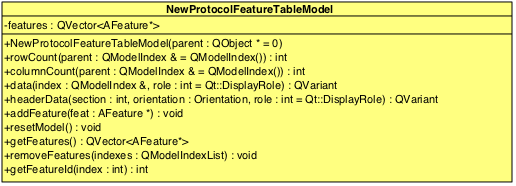
\includegraphics[width=0.6\linewidth]{./Content/Immagini/QtModel/NewProtocolFeatureTableModel.png}
	\caption{Diagramme classe \textsl{NewProtocolFeatureTableModel}}
	\label{comp_NewProtocolFeatureTableModel}
\end{figure}

\paragraph{Descrizione\\} 
Classe che rappresenta il model della tabella delle feature\g{} presente nella vista di creazione dei protocol\g{}.

\paragraph{Utilizzo\\}
La classe viene utilizzata come model dalla tabella delle feature\g{} della vista di creazione dei protocol\g{}.

\paragraph{Classi ereditate:}
\begin{itemize}
	\item Romeo::Model::QtModel::TableModel.
\end{itemize}

\paragraph{\textcolor{black}{Attributi\\}}
	\begin{itemize}
		\item \color{teal}\verb!- features : QVector<AFeature*>!
		\color{black}
		\subparagraph{Descrizione:} È il vettore delle feature\g{} che compone il model.
	\end{itemize}
	
\paragraph{\color{black}Metodi\\}
\begin{itemize}
	\item \color{blue}\verb!+ NewProtocolFeatureTableModel(parent : QObject*)!\\
		\color{black}
		\subparagraph{Descrizione:} costruttore della classe.\\
		\subparagraph{Argomenti}
			\begin{itemize}
				\item \color{RoyalPurple}\verb!parent : QObject*!\\
				\color{Black}Parente dell'oggetto NewProtocolFeatureTableModel.
			\end{itemize}
			
	\item \color{blue}\verb!+ rowCount(parent : const QModelIndex &) : int!\\
	\color{black}
	\subparagraph{Descrizione:} metodo virtuale che ha come contratto il conteggio di numero di righe e lo ritorna.
	\\Il metodo viene invocato automaticamente da Qt\g{} nella generazione del Model.\\
	\subparagraph{Argomenti}
		\begin{itemize}
			\item \color{RoyalPurple}\verb!parent : const QModelIndex &!\\
			\color{Black}Rappresenta l'indice attuale del model.
		\end{itemize}
	\subparagraph{Note}
			\begin{itemize}
				\item Il metodo è costante.
			\end{itemize}
	
	\item \color{blue}\verb!+ columnCount(parent : const QModelIndex &) : int!\\
	\color{black}
	\subparagraph{Descrizione:} metodo virtuale che ha come contratto il conteggio di numero di colonne e lo ritorna.\\
	Il metodo viene invocato automaticamente da Qt\g{} nella generazione del Model.\\
	Il metodo deve essere ridefinito nelle classi che ereditano da questa.\\
	\subparagraph{Argomenti}
		\begin{itemize}
			\item \color{RoyalPurple}\verb! parent : const QModelIndex &!\\
			\color{black}Rappresenta l'indice attuale del model.
		\end{itemize}
	\subparagraph{Note}
			\begin{itemize}
				\item Il metodo è costante.
			\end{itemize}
		
	\item \color{blue}\verb! + data(index : const QModelIndex &, !\\
					\verb!role: int) : QVariant!\\
	\color{black}
	\subparagraph{Descrizione:} metodo virtuale che ha come contratto l'inserimento dei dati nella riga della tabella, ritorna il testo da inserire nelle singole celle\\
		Il metodo viene invocato automaticamente da Qt\g{} nella generazione del Model.\\
		Il metodo deve essere ridefinito nelle classi che ereditano da questa.\\
	\subparagraph{Argomenti}
		\begin{itemize}
			\item \color{RoyalPurple}\verb! parent : const QModelIndex &!\\
			\color{black}Rappresena l'indice attuale del model;
			
			\item \color{RoyalPurple}\verb! role : int!\\
			\color{black}Regola di visualizzazione Qt\g{}.
		\end{itemize}
	\subparagraph{Note}
			\begin{itemize}
				\item Il metodo è costante.
			\end{itemize}
		
	\item \color{blue}\verb!+ headerData(section : int, orientation : Qt::Orientation,!\\
	  \verb!role : int) : QVariant!\\
	\color{black}
	\subparagraph{Descrizione:} metodo virtuale che ha come contratto l'inserimento delle intestazioni della tabella, ritorna il testo da inserire in ogni intestazione.\\
	Il metodo viene invocato automaticamente da Qt\g{} nella generazione del Model.\\
	Il metodo deve essere ridefinito nelle classi che ereditano da questa.\\
	\subparagraph{Argomenti}
		\begin{itemize}
			\item \color{RoyalPurple}\verb! section : int!\\
			\color{black}Rappresenta l'indice della colonna o riga in base all'orientamento;
			
			\item \color{RoyalPurple}\verb! orientation : Qt::Orientation!\\
			\color{black}Rappresenta l'orientamento della tabella;
			
			\item \color{RoyalPurple}\verb! role : int!\\
			\color{black}Regola di visualizzazione Qt\g{}.
		\end{itemize}
	\subparagraph{Note}
			\begin{itemize}
				\item Il metodo è costante.
			\end{itemize}
		
	\item \color{blue}\verb!+ addFeature(feat : AFeature*) : void!\\
		\color{black}
		\subparagraph{Descrizione:} Il metodo aggiunge la feature\g{} al model.\\
		\subparagraph{Argomenti}
			\begin{itemize}				
				\item \color{RoyalPurple}\verb! feat : AFeature*!\\
				\color{black} È la feature\g{} da aggiungere.
			\end{itemize}
			
	\item \color{blue}\verb!+ resetModel() : void!\\
		\color{black}
		\subparagraph{Descrizione:} Il metodo svuota il model.\\
		
	\item \color{blue}\verb!+ getFeatures() : QVector<AFeature*>!\\
		\color{black}
		\subparagraph{Descrizione:} Il metodo ritorna il vettore di tutte le feature\g{} del model.\\
		\subparagraph{Note}
				\begin{itemize}
					\item Il metodo è costante.
				\end{itemize}
		
	\item \color{blue}\verb!+ removeFeatures(indexes : QModelIndexList) : void!\\
		\color{black}
		\subparagraph{Descrizione:} Il metodo rimuove le feature\g{} puntate dagli indici dal model.\\
		\subparagraph{Argomenti}
			\begin{itemize}				
				\item \color{RoyalPurple}\verb! indexes : QModelIndexList!\\
				\color{black} È la lista degli indici della tabella.
			\end{itemize}
			
	\item \color{blue}\verb!+ getFeatureId(index : int) : void!\\
		\color{black}
		\subparagraph{Descrizione:} Il metodo ritorna l'ID della feature\g{} nella posizione index del vettore del model.\\
		\subparagraph{Argomenti}
			\begin{itemize}				
				\item \color{RoyalPurple}\verb! index : int!\\
				\color{black} È la posizione del vettore.
			\end{itemize}
		\subparagraph{Note}
				\begin{itemize}
					\item Il metodo è costante.
				\end{itemize}
\end{itemize}
\pagebreak

% % % % % % % % % % % % % % % % % %

\subsubsection{ProtocolTableModel(class)}
\label{ProtocolTableModel}
\begin{figure}[!h]
	\centering
	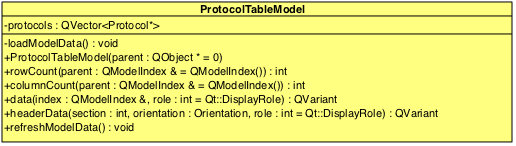
\includegraphics[width=0.6\linewidth]{./Content/Immagini/QtModel/ProtocolTableModel.png}
	\caption{Diagramma classe \textsl{ProtocolTableModel}}
	\label{comp_ProtocolTableModel}
\end{figure}

\paragraph{Descrizione\\} 
Classe che rappresenta il model della tabella dei protocol\g{} presente nella vista di visualizzazione dei protocol\g{}.

\paragraph{Utilizzo\\}
La classe viene utilizzata come model dalla tabella dei protocol\g{} della vista di visualizzazione dei protocol\g{}.

\paragraph{Classi ereditate:}
\begin{itemize}
	\item Romeo::Model::QtModel::TableModel.
\end{itemize}

\paragraph{\textcolor{black}{Attributi\\}}
	\begin{itemize}
		\item \color{teal}\verb!- protocols : QVector<Protocol*>!
		\color{black}
		\subparagraph{Descrizione:} È il vettore dei protocol\g{} che compone il model.
	\end{itemize}
	
\paragraph{\color{black}Metodi\\}
\begin{itemize}
	\item \color{blue}\verb!+ ProtocolTableModel(parent : QObject*)!\\
		\color{black}
		\subparagraph{Descrizione:} costruttore della classe.\\
		\subparagraph{Argomenti}
			\begin{itemize}
				\item \color{RoyalPurple}\verb!parent : QObject*!\\
				\color{Black}Parente dell'oggetto ProtocolTableModel.
			\end{itemize}
			
	\item \color{blue}\verb!+ rowCount(parent : const QModelIndex &) : int!\\
	\color{black}
	\subparagraph{Descrizione:} metodo virtuale che ha come contratto il conteggio di numero di righe e lo ritorna.
	\\Il metodo viene invocato automaticamente da Qt\g{} nella generazione del Model.\\
	\subparagraph{Argomenti}
		\begin{itemize}
			\item \color{RoyalPurple}\verb!parent : const QModelIndex &!\\
			\color{Black}Rappresenta l'indice attuale del model.
		\end{itemize}
	\subparagraph{Note}
			\begin{itemize}
				\item Il metodo è costante.
			\end{itemize}
	
	\item \color{blue}\verb!+ columnCount(parent : const QModelIndex &) : int!\\
	\color{black}
	\subparagraph{Descrizione:} metodo virtuale che ha come contratto il conteggio di numero di colonne e lo ritorna.\\
	Il metodo viene invocato automaticamente da Qt\g{} nella generazione del Model.\\
	Il metodo deve essere ridefinito nelle classi che ereditano da questa.\\
	\subparagraph{Argomenti}
		\begin{itemize}
			\item \color{RoyalPurple}\verb! parent : const QModelIndex &!\\
			\color{black}Rappresenta l'indice attuale del model.
		\end{itemize}
	\subparagraph{Note}
			\begin{itemize}
				\item Il metodo è costante.
			\end{itemize}
		
	\item \color{blue}\verb! + data(index : const QModelIndex &, !\\
					\verb!role: int) : QVariant!\\
	\color{black}
	\subparagraph{Descrizione:} metodo virtuale che ha come contratto l'inserimento dei dati nella riga della tabella, ritorna il testo da inserire nelle singole celle\\
		Il metodo viene invocato automaticamente da Qt\g{} nella generazione del Model.\\
		Il metodo deve essere ridefinito nelle classi che ereditano da questa.\\
	\subparagraph{Argomenti}
		\begin{itemize}
			\item \color{RoyalPurple}\verb! parent : const QModelIndex &!\\
			\color{black}Rappresena l'indice attuale del model;
			
			\item \color{RoyalPurple}\verb! role : int!\\
			\color{black}Regola di visualizzazione Qt\g{}.
		\end{itemize}
	\subparagraph{Note}
			\begin{itemize}
				\item Il metodo è costante.
			\end{itemize}
		
	\item \color{blue}\verb!+ headerData(section : int, orientation : Qt::Orientation,!\\
	  \verb!role : int) : QVariant!\\
	\color{black}
	\subparagraph{Descrizione:} metodo virtuale che ha come contratto l'inserimento delle intestazioni della tabella, ritorna il testo da inserire in ogni intestazione.\\
	Il metodo viene invocato automaticamente da Qt\g{} nella generazione del Model.\\
	Il metodo deve essere ridefinito nelle classi che ereditano da questa.\\
	\subparagraph{Argomenti}
		\begin{itemize}
			\item \color{RoyalPurple}\verb! section : int!\\
			\color{black}Rappresenta l'indice della colonna o riga in base all'orientamento;
			
			\item \color{RoyalPurple}\verb! orientation : Qt::Orientation!\\
			\color{black}Rappresenta l'orientamento della tabella;
			
			\item \color{RoyalPurple}\verb! role : int!\\
			\color{black}Regola di visualizzazione Qt\g{}.
		\end{itemize}
	\subparagraph{Note}
			\begin{itemize}
				\item Il metodo è costante.
			\end{itemize}
		
	\item \color{blue}\verb!+ refreshModelData() : void!\\
		\color{black}
		\subparagraph{Descrizione:} Ricarica i dati del model.\\
			
	\item \color{blue}\verb!- loadModelData() : void!\\
		\color{black}
		\subparagraph{Descrizione:} Carica i dati del model .\\
\end{itemize}
\pagebreak

% % % % % % % % % % % % % % % % % %

\subsubsection{ResultsTableModel(class)}
\label{ResultsTableModel}
\begin{figure}[!h]
	\centering
	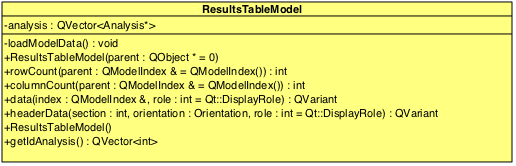
\includegraphics[width=0.6\linewidth]{./Content/Immagini/QtModel/ResultsTableModel.png}
	\caption{Diagramma classe \textsl{ResultsTableModel}}
	\label{comp_ResultsTableModel}
\end{figure}

\paragraph{Descrizione\\} 
Classe che rappresenta il model della tabella delle analisi effettuate presente nella vista di visualizzazione delle analisi.

\paragraph{Utilizzo\\}
La classe viene utilizzata come model dalla tabella delle analisi effettuate della vista di visualizzazione analisi.

\paragraph{Classi ereditate:}
\begin{itemize}
	\item Romeo::Model::QtModel::TableModel.
\end{itemize}

\paragraph{\textcolor{black}{Attributi\\}}
	\begin{itemize}
		\item \color{teal}\verb!- analysis : QVector<Analysis*>!
		\color{black}
		\subparagraph{Descrizione:} È il vettore di analisi che compone il model.
	\end{itemize}
	
\paragraph{\color{black}Metodi\\}
\begin{itemize}
	\item \color{blue}\verb!+ ResultsTableModel(parent : QObject*)!\\
		\color{black}
		\subparagraph{Descrizione:} costruttore della classe.\\
		\subparagraph{Argomenti}
			\begin{itemize}
				\item \color{RoyalPurple}\verb!parent : QObject*!\\
				\color{Black}Parente dell'oggetto ResultsTableModel.
			\end{itemize}
			
	\item \color{blue}\verb!+ rowCount(parent : const QModelIndex &) : int!\\
	\color{black}
	\subparagraph{Descrizione:} metodo virtuale che ha come contratto il conteggio di numero di righe e lo ritorna.
	\\Il metodo viene invocato automaticamente da Qt\g{} nella generazione del Model.\\
	\subparagraph{Argomenti}
		\begin{itemize}
			\item \color{RoyalPurple}\verb!parent : const QModelIndex &!\\
			\color{Black}Rappresenta l'indice attuale del model.
		\end{itemize}
	\subparagraph{Note}
			\begin{itemize}
				\item Il metodo è costante.
			\end{itemize}
	
	\item \color{blue}\verb!+ columnCount(parent : const QModelIndex &) : int!\\
	\color{black}
	\subparagraph{Descrizione:} metodo virtuale che ha come contratto il conteggio di numero di colonne e lo ritorna.\\
	Il metodo viene invocato automaticamente da Qt\g{} nella generazione del Model.\\
	Il metodo deve essere ridefinito nelle classi che ereditano da questa.\\
	\subparagraph{Argomenti}
		\begin{itemize}
			\item \color{RoyalPurple}\verb! parent : const QModelIndex &!\\
			\color{black}Rappresenta l'indice attuale del model.
		\end{itemize}
	\subparagraph{Note}
			\begin{itemize}
				\item Il metodo è costante.
			\end{itemize}
		
	\item \color{blue}\verb! + data(index : const QModelIndex &, !\\
					\verb!role: int) : QVariant!\\
	\color{black}
	\subparagraph{Descrizione:} metodo virtuale che ha come contratto l'inserimento dei dati nella riga della tabella, ritorna il testo da inserire nelle singole celle\\
		Il metodo viene invocato automaticamente da Qt\g{} nella generazione del Model.\\
		Il metodo deve essere ridefinito nelle classi che ereditano da questa.\\
	\subparagraph{Argomenti}
		\begin{itemize}
			\item \color{RoyalPurple}\verb! parent : const QModelIndex &!\\
			\color{black}Rappresena l'indice attuale del model;
			
			\item \color{RoyalPurple}\verb! role : int!\\
			\color{black}Regola di visualizzazione Qt\g{}.
		\end{itemize}
	\subparagraph{Note}
			\begin{itemize}
				\item Il metodo è costante.
			\end{itemize}
		
	\item \color{blue}\verb!+ headerData(section : int, orientation : Qt::Orientation,!\\
	  \verb!role : int) : QVariant!\\
	\color{black}
	\subparagraph{Descrizione:} metodo virtuale che ha come contratto l'inserimento delle intestazioni della tabella, ritorna il testo da inserire in ogni intestazione.\\
	Il metodo viene invocato automaticamente da Qt\g{} nella generazione del Model.\\
	Il metodo deve essere ridefinito nelle classi che ereditano da questa.\\
	\subparagraph{Argomenti}
		\begin{itemize}
			\item \color{RoyalPurple}\verb! section : int!\\
			\color{black}Rappresenta l'indice della colonna o riga in base all'orientamento;
			
			\item \color{RoyalPurple}\verb! orientation : Qt::Orientation!\\
			\color{black}Rappresenta l'orientamento della tabella;
			
			\item \color{RoyalPurple}\verb! role : int!\\
			\color{black}Regola di visualizzazione Qt\g{}.
		\end{itemize}
	\subparagraph{Note}
			\begin{itemize}
				\item Il metodo è costante.
			\end{itemize}
		
	\item \color{blue}\verb!+ getIdAnalysis() : QVector<int>!\\
		\color{black}
		\subparagraph{Descrizione:} Ritorna gli ID delle analisi presenti nel model.\\
		\subparagraph{Note}
				\begin{itemize}
					\item Il metodo è costante.
				\end{itemize}
			
	\item \color{blue}\verb!- loadModelData() : void!\\
		\color{black}
		\subparagraph{Descrizione:} Carica i dati del model .\\
\end{itemize}
\pagebreak

% % % % % % % % % % % % % % % % % %

\subsubsection{SubjectTableModel(class)}
\label{SubjectTableModel}
\begin{figure}[!h]
	\centering
	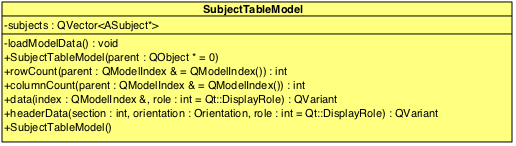
\includegraphics[width=0.6\linewidth]{./Content/Immagini/QtModel/SubjectTableModel.png}
	\caption{Diagramma classe \textsl{SubjectTableModel}}
	\label{comp_SubjectTableModelv}
\end{figure}

\paragraph{Descrizione\\} 
Classe che rappresenta il model della tabella dei subject\g{} presente nella vista di visualizzazione dei subject\g{}.

\paragraph{Utilizzo\\}
La classe viene utilizzata come model dalla tabella dei subject\g{} della vista di visualizzazione subject\g{}.

\paragraph{Classi ereditate:}
\begin{itemize}
	\item Romeo::Model::QtModel::TableModel.
\end{itemize}

\paragraph{\textcolor{black}{Attributi\\}}
	\begin{itemize}
		\item \color{teal}\verb!- subjects : QVector<ASubject*>!
			\color{black}
			\subparagraph{Descrizione:} È il vettore di subject\g{} che compone il model.
	\end{itemize}
	
\paragraph{\color{black}Metodi\\}
\begin{itemize}
	\item \color{blue}\verb!+ SubjectTableModel(parent : QObject*)!\\
		\color{black}
		\subparagraph{Descrizione:} costruttore della classe.\\
		\subparagraph{Argomenti}
			\begin{itemize}
				\item \color{RoyalPurple}\verb!parent : QObject*!\\
				\color{Black}Parente dell'oggetto SubjectTableModel.
			\end{itemize}
			
	\item \color{blue}\verb!+ rowCount(parent : const QModelIndex &) : int!\\
	\color{black}
	\subparagraph{Descrizione:} metodo virtuale che ha come contratto il conteggio di numero di righe e lo ritorna.
	\\Il metodo viene invocato automaticamente da Qt\g{} nella generazione del Model.\\
	\subparagraph{Argomenti}
		\begin{itemize}
			\item \color{RoyalPurple}\verb!parent : const QModelIndex &!\\
			\color{Black}Rappresenta l'indice attuale del model.
		\end{itemize}
	\subparagraph{Note}
			\begin{itemize}
				\item Il metodo è costante.
			\end{itemize}
	
	\item \color{blue}\verb!+ columnCount(parent : const QModelIndex &) : int!\\
	\color{black}
	\subparagraph{Descrizione:} metodo virtuale che ha come contratto il conteggio di numero di colonne e lo ritorna.\\
	Il metodo viene invocato automaticamente da Qt\g{} nella generazione del Model.\\
	Il metodo deve essere ridefinito nelle classi che ereditano da questa.\\
	\subparagraph{Argomenti}
		\begin{itemize}
			\item \color{RoyalPurple}\verb! parent : const QModelIndex &!\\
			\color{black}Rappresenta l'indice attuale del model.
		\end{itemize}
	\subparagraph{Note}
			\begin{itemize}
				\item Il metodo è costante.
			\end{itemize}
		
	\item \color{blue}\verb! + data(index : const QModelIndex &, !\\
					\verb!role: int) : QVariant!\\
	\color{black}
	\subparagraph{Descrizione:} metodo virtuale che ha come contratto l'inserimento dei dati nella riga della tabella, ritorna il testo da inserire nelle singole celle\\
		Il metodo viene invocato automaticamente da Qt\g{} nella generazione del Model.\\
		Il metodo deve essere ridefinito nelle classi che ereditano da questa.\\
	\subparagraph{Argomenti}
		\begin{itemize}
			\item \color{RoyalPurple}\verb! parent : const QModelIndex &!\\
			\color{black}Rappresena l'indice attuale del model;
			
			\item \color{RoyalPurple}\verb! role : int!\\
			\color{black}Regola di visualizzazione Qt\g{}.
		\end{itemize}
	\subparagraph{Note}
			\begin{itemize}
				\item Il metodo è costante.
			\end{itemize}
		
	\item \color{blue}\verb!+ headerData(section : int, orientation : Qt::Orientation,!\\
	  \verb!role : int) : QVariant!\\
	\color{black}
	\subparagraph{Descrizione:} metodo virtuale che ha come contratto l'inserimento delle intestazioni della tabella, ritorna il testo da inserire in ogni intestazione.\\
	Il metodo viene invocato automaticamente da Qt\g{} nella generazione del Model.\\
	Il metodo deve essere ridefinito nelle classi che ereditano da questa.\\
	\subparagraph{Argomenti}
		\begin{itemize}
			\item \color{RoyalPurple}\verb! section : int!\\
			\color{black}Rappresenta l'indice della colonna o riga in base all'orientamento;
			
			\item \color{RoyalPurple}\verb! orientation : Qt::Orientation!\\
			\color{black}Rappresenta l'orientamento della tabella;
			
			\item \color{RoyalPurple}\verb! role : int!\\
			\color{black}Regola di visualizzazione Qt\g{}.
		\end{itemize}
	\subparagraph{Note}
			\begin{itemize}
				\item Il metodo è costante.
			\end{itemize}
		
	\item \color{blue}\verb!- loadModelData() : void!\\
		\color{black}
		\subparagraph{Descrizione:} Carica i dati del model .\\
\end{itemize}

% % % % % % % % % % % % % % % % % %																											